\chapter{Applications of the Photon}

\setcounter{section}{6}
\setcounter{subsection}{0}
\setcounter{subsubsection}{1}
\setcounter{secnumdepth}{3}
% Define box styles
\tcbset{physikbox/.style={colback=blue!5!white, colframe=blue!75!black, fonttitle=\bfseries}}
\tcbset{mathebox/.style={colback=green!5!white, colframe=green!50!black, fonttitle=\bfseries}}
\tcbset{didaktikbox/.style={colback=yellow!5!white, colframe=yellow!50!black, fonttitle=\bfseries}}
\tcbset{hypobox/.style={colback=orange!5!white, colframe=orange!75!black, fonttitle=\bfseries}}
\tcbset{hinweisbox/.style={colback=gray!10!white, colframe=black!40!black, fonttitle=\bfseries}}

\subsection{Introduction}

Photons\index{Photon} are not only fundamental carriers of quantum-physical properties\index{Quantum-Physical Property} – they also form the basis of countless applications\index{Application} in technology\index{Technology}, research\index{Research}, and everyday life.  
This chapter presents selected fields of use where the control\index{Photon Control}, detection\index{Photon Detection}, and utilization\index{Photon Utilization} of individual photons play a central role.  
The range extends from laser technology\index{Laser Technology} and quantum sensing\index{Quantum Sensing} to medical imaging\index{Medical Imaging}, optical communication\index{Optical Communication}, and astronomical observation\index{Astronomical Observation}.  
The goal is to make the physical principles\index{Physical Principle} behind these applications understandable and to show their significance for science\index{Science} and society.\index{Society}

\subsection{Photons in Laser Technology}
\subsubsection{Operating Principle of Lasers}

The term “laser”\index{Laser} stands for \textbf{Light Amplification by Stimulated Emission of Radiation}\index{Light Amplification by Stimulated Emission of Radiation}.  
A laser does not produce light\index{Light} through incandescence\index{Incandescence} or chemical reactions\index{Chemical Reaction}, but by the controlled amplification of photons in an active medium\index{Active Medium} – based on the principle of \emph{stimulated emission}\index{Stimulated Emission}.

\noindent
The three central processes\index{Einstein Processes}, theoretically described by Einstein\index{Einstein, Albert} already in 1916, are:

\begin{itemize}
	\item \textbf{Spontaneous emission}\index{Spontaneous Emission}: An excited atom\index{Atom} decays to a lower state without external influence and emits a photon.
	\item \textbf{Absorption}\index{Absorption}: A photon excites an atom in the ground state to a higher energy state.
	\item \textbf{Stimulated emission}: A photon interacts with an already excited atom – which then emits a second photon, phase-coherent with the first.
\end{itemize}

For effective light amplification\index{Light Amplification}, stimulated emission must dominate. This requires a so-called \emph{population inversion}\index{Population Inversion} – i.e., more atoms in the excited than in the ground state, which under normal conditions is not the case.

\vspace{1em}
\begin{tcolorbox}[physikbox, title={Stimulated Emission as the Basis of Lasers}]
	\label{box:grundlagedeslaser}
	If a photon of the right energy strikes an excited atom, it can force the atom to emit a second photon. Both photons are:
	\begin{itemize}
		\item \textbf{phase-coherent}\index{Phase Coherence} (same wave phase),
		\item \textbf{frequency-identical}\index{Frequency Identity} (same energy), and
		\item \textbf{propagating in the same direction}\index{Propagation Direction}.
	\end{itemize}
	This property enables the controlled amplification of light – the operating principle of the laser.
\end{tcolorbox}

\subsubsection{Structure and Types}

A laser essentially consists of three functional components:

\begin{itemize}
	\item \textbf{Active medium:} A material\index{Laser Material} whose atoms or molecules\index{Molecule} can be brought into excited states by energy supply (pumping\index{Pumping}). This is where stimulated emission occurs.
	\item \textbf{Pump unit}\index{Pump Unit}: Provides the necessary energy to achieve a population inversion. Possible methods include optical\index{Optical Pumping}, electrical\index{Electrical Pumping}, or chemical pumping\index{Chemical Pumping}.
	\item \textbf{Resonator}\index{Resonator}: Two mirrors\index{Mirror} that reflect light back and forth. One mirror is partially transparent\index{Partially Reflective Mirror}, allowing part of the amplified light to exit as the laser beam\index{Laser Beam}.
\end{itemize}
\newpage
\noindent
\begin{tcolorbox}[didaktikbox, title={Variety of Laser Types – An Overview}]
	\label{box:Typenvielfalt von Lasern}
	Lasers are mainly distinguished by their active medium:
	\begin{itemize}
		\item \textbf{Solid-state lasers}\index{Solid-State Laser} (e.g., Nd:YAG\index{Nd:YAG}): High power, used in industry\index{Industry} and medicine\index{Medicine}.
		\item \textbf{Gas lasers}\index{Gas Laser} (e.g., helium–neon\index{Helium–Neon Laser}, CO\textsubscript{2}\index{CO2 Laser}): Stable and precise, e.g., for surveying\index{Surveying}.
		\item \textbf{Semiconductor lasers}\index{Semiconductor Laser} (e.g., laser diode\index{Laser Diode}): Compact, efficient, e.g., in CD/DVD players\index{CD Player}\index{DVD Player} or laser pointers\index{Laser Pointer}.
		\item \textbf{Fiber lasers}\index{Fiber Laser}: Amplify light in an optical fiber\index{Optical Fiber} – high beam quality\index{Beam Quality} with robust design.
		\item \textbf{Dye lasers}\index{Dye Laser}: Particularly flexible in wavelength\index{Wavelength}, using organic molecules\index{Organic Molecule} as medium.
	\end{itemize}
\end{tcolorbox}

\subsubsection{Applications in Technology and Research}

\begin{tcolorbox}[didaktikbox, title={Applications of Lasers — Technology (Overview)}]	
	\label{box:lasertechnik}
	\begin{itemize}
		\item \textbf{Materials processing\index{Materials Processing} (cutting, welding, hardening):} High power density, precise focus, narrow heat-affected zone, easily automated.
		\item \textbf{Additive manufacturing\index{Additive Manufacturing} (SLS/SLM, PBF):} Point-by-point melting for complex, high-strength parts with minimal material use.
		\item \textbf{Measurement technology\index{Measurement Technology} \& metrology\index{Metrology} (interferometry, laser tracker):} Precision length/angle measurements down to the nanometer scale due to coherence and stability.
		\item \textbf{LIDAR\index{LIDAR} \& distance measurement\index{Distance Measurement}:} Fast 3D mapping and robust ranging (autonomous driving, drones, geodesy).
		\item \textbf{Fiber-optic communication\index{Fiber-Optic Communication}:} Very high data rates over long distances (DWDM, coherent transmission).
		\item \textbf{Surface structuring\index{Surface Structuring} \& lithography\index{Lithography}:} Direct micro-/nanopatterning (“laser direct write”), prototyping, micromechanics.
		\item \textbf{Process analytics\index{Process Analytics} (Raman\index{Raman Spectroscopy}, LIBS\index{LIBS}):} Contactless, fast material sensing inline without sample prep.
		\item \textbf{Holography\index{Holography}, displays\index{Display} \& projection\index{Projection}:} High contrast, wide color gamut, real holograms and AR optics.
		\item \textbf{Barcode scanning\index{Barcode Scanning} \& sensors\index{Sensor}:} Fast, high-contrast scanning in retail, logistics, and automation.
		\item \textbf{Alignment\index{Alignment} \& adjustment\index{Adjustment}:} The laser beam as a precise reference line in construction and mechanical engineering.
	\end{itemize}
\end{tcolorbox}

\begin{tcolorbox}[didaktikbox, title={Applications of Lasers — Research (Overview)}] 
	\label{box:laser-app-forschung}
	\begin{itemize}
		\item \textbf{Spectroscopy\index{Spectroscopy} (absorption, fluorescence, Raman, CARS):} Narrowband/tunable with high selectivity for structural and molecular information.
		\item \textbf{Optical tweezers\index{Optical Tweezer} \& micromanipulation\index{Micromanipulation}:} Contactless control of particles or cells using strongly focused beams.
		\item \textbf{Atomic physics\index{Atomic Physics} (laser cooling\index{Laser Cooling}, MOT\index{Magneto-Optical Trap}, BEC\index{Bose–Einstein Condensate}):} Resonant cooling down to nK and precise control of neutral atoms.
		\item \textbf{Precision metrology\index{Precision Metrology} (optical clocks\index{Optical Clock}, frequency combs\index{Frequency Comb}):} Extremely stable frequencies and new time/length standards.
		\item \textbf{Nonlinear optics\index{Nonlinear Optics} \& attosecond physics\index{Attosecond Physics}:} Frequency conversion, high harmonics, and ultrafast dynamics.
		\item \textbf{Quantum optics\index{Quantum Optics} \& quantum communication\index{Quantum Communication} (QKD\index{Quantum Key Distribution}):} Single photons, entanglement, secure key distribution.
		\item \textbf{Laser–plasma\index{Laser Plasma}, accelerators\index{Particle Accelerator}, fusion\index{Nuclear Fusion}:} Extreme intensities for dense plasmas, compact accelerators, and inertial confinement fusion.
		\item \textbf{Atmosphere\index{Atmosphere} \& astronomy\index{Astronomy} (lidar, laser guide stars\index{Laser Guide Star}):} Probing aerosols/winds; adaptive optics for large telescopes.
		\item \textbf{Biomedical imaging\index{Biomedical Imaging} (two-photon, STED\index{STED Microscopy}):} Deep, gentle, and super-resolution microscopy.
		\item \textbf{Femtochemistry\index{Femtochemistry} \& pump–probe\index{Pump–Probe Experiment}:} Making reaction dynamics visible in real time.
	\end{itemize}
\end{tcolorbox}

\subsection{Photon Detectors and Sensing\index{Photon detectors}\index{Sensing}}

The detection of individual photons\index{Photon} is a key technology in modern physics and engineering. Whether in astrophysics\index{Astrophysics}, quantum optics\index{Quantum optics}, medical imaging\index{Medical imaging}, or industrial quality control\index{Quality control} – sensitive and precise sensors determine the reliability of an experiment or the success of an application. This section introduces central types of photon detectors, their operating principles, and typical applications.

\subsubsection{Photomultipliers and Semiconductor Detectors\index{Photomultiplier}\index{Semiconductor detectors}}

\textbf{Photomultiplier tubes (PMTs)\index{PMT}} exploit the photoelectric effect\index{Photoelectric effect}: An incoming photon knocks an electron out of a photocathode\index{Photocathode}. This electron is multiplied in a cascade of dynodes\index{Dynode} and detected as a macroscopically measurable electrical signal. PMTs offer:

\begin{itemize}
	\item high gain (up to $10^6$–$10^8$),
	\item extremely high sensitivity in the UV\index{Ultraviolet} to visible range,
	\item fast response times in the nanosecond range.
\end{itemize}

Disadvantages include sensitivity to magnetic fields\index{Magnetic field}, the requirement of high voltage\index{High voltage}, and the mechanical fragility of the glass tubes.

\medskip

\textbf{Semiconductor detectors\index{Semiconductor detectors}}, in particular avalanche photodiodes (APDs\index{APD}) and single-photon avalanche diodes (SPADs\index{SPAD}), also work via the photoelectric effect, but within a semiconductor material\index{Semiconductor material}. Advantages:

\begin{itemize}
	\item compact design, robust, and easily integrable,
	\item good quantum efficiency\index{Quantum efficiency} (often exceeding 50\%),
	\item possibility of array integration\index{Array integration} (pixel detectors, SiPMs\index{SiPM}).
\end{itemize}
\newpage
\noindent
They are the foundation of modern photonic sensor arrays\index{Sensor array} in research and industry.
\begin{figure}[H]
	\centering
	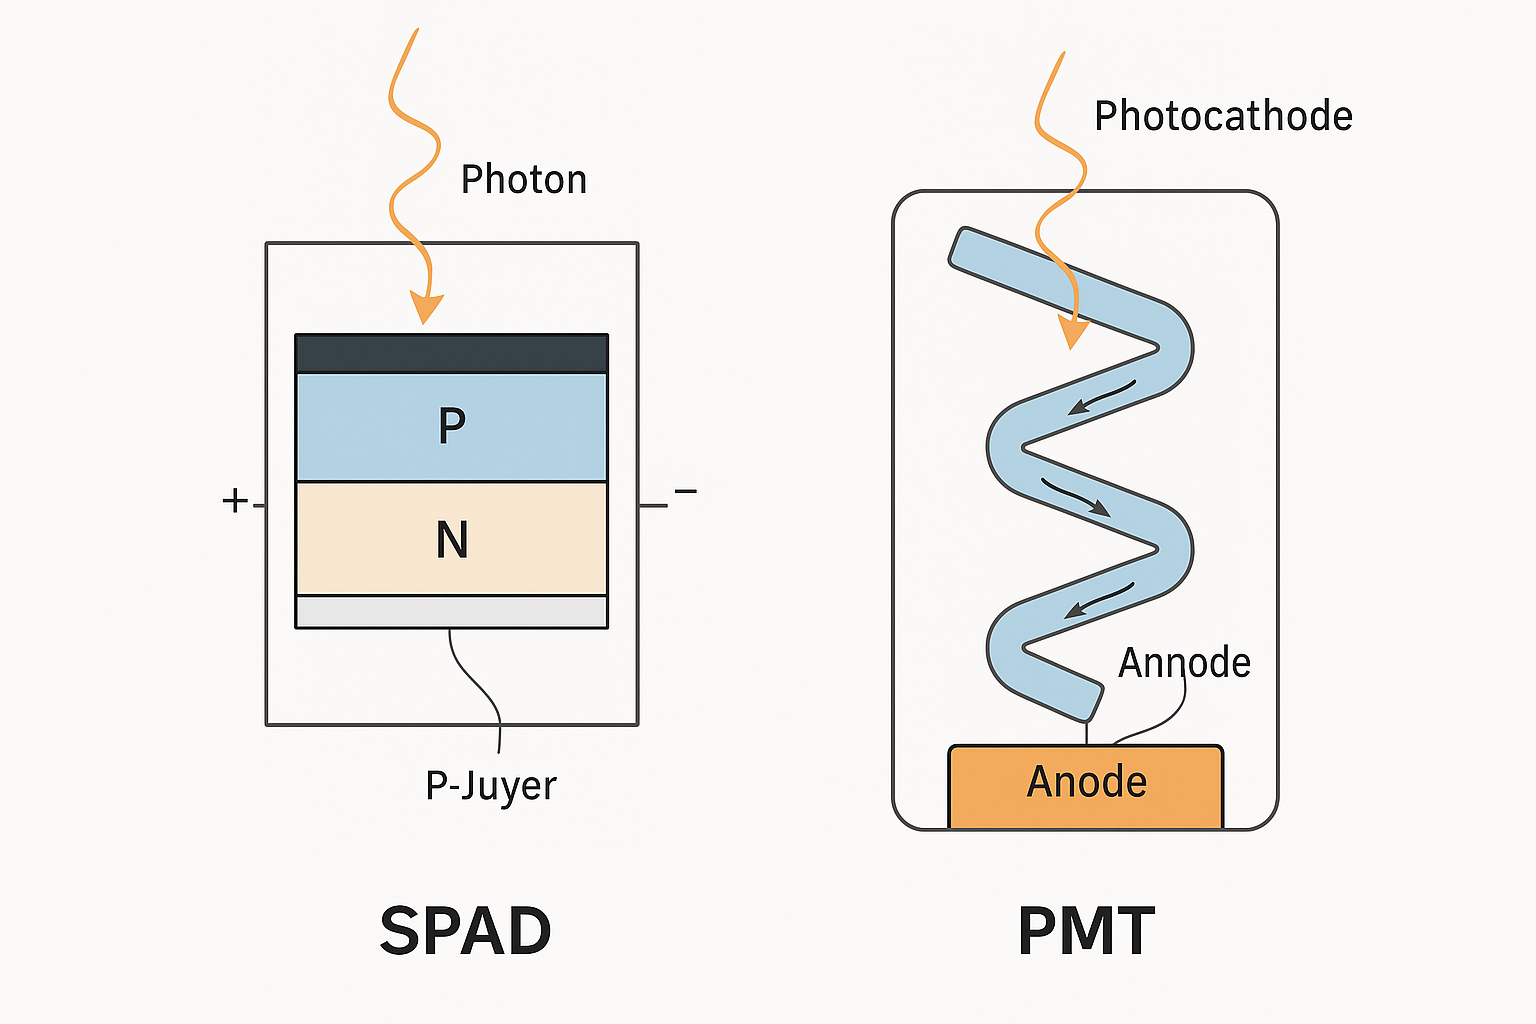
\includegraphics[width=0.9\textwidth]{bilder/SPAD-PMT.png}
	\caption{Schematic comparison of a SPAD (Single-Photon Avalanche Diode, left) and a PMT (Photomultiplier Tube, right). }
	\label{fig:spad_pmt}
\end{figure}
\begin{tcolorbox}[hinweisbox, title=Didactic Comparison: SPAD vs. PMT]
	\label{box:vergleich SPAD}
	\small
	\begin{tabular}{p{0.48\textwidth} | p{0.48\textwidth}}
		\textbf{Single-Photon Avalanche Diode (SPAD)} & \textbf{Photomultiplier Tube (PMT)} \\
		\hline
		Semiconductor device with a special PN junction\index{PN junction}. & Vacuum tube\index{Vacuum tube} with photocathode and amplification stages. \\
		\hline
		A photon generates an electron–hole pair\index{Electron–hole pair} in the depletion region\index{Depletion region}. & A photon knocks an electron out of the photocathode. \\
		\hline
		The electron triggers an avalanche breakdown\index{Avalanche breakdown} – producing an electrical pulse. & The electron is accelerated and multiplied across multiple dynodes. \\
		\hline
		Very high time resolution\index{Time resolution}, ideal for compact, integrated quantum sensors\index{Quantum sensor}. & High gain, ideal for weak light sources (e.g., scintillators\index{Scintillator}). \\
		\hline
		Operates at room temperature\index{Room temperature}, easily integrated into chips\index{Chip}. & Requires high voltage, sensitive to magnetic fields. \\
		\hline
		Well suited for arrays and imaging systems (SiPM). & Traditionally used in nuclear physics\index{Nuclear physics}, astronomy, PET\index{Positron emission tomography}, etc. \\
	\end{tabular}
\end{tcolorbox}
\begin{tcolorbox}[didaktikbox, title=Concept: Avalanche Breakdown]
	\label{box:avalanche}
	\small
	In an \textbf{avalanche breakdown}, a free electron in the strong electric field\index{Electric field} of a semiconductor generates additional electrons through impact ionization\index{Impact ionization}. This process multiplies like an avalanche and produces a measurable current pulse\index{Current pulse} – enabling the detection of a single photon.
\end{tcolorbox}
\vspace{1em}
\begin{tcolorbox}[didaktikbox, title=Concept: Scintillator]
	\label{box:szintillator}
	\small
	A \textbf{scintillator} is a material\index{Material} that emits light\index{Light} when struck by ionizing particles\index{Ionizing particle}. This so-called \emph{scintillation light}\index{Scintillation light} can be registered by photon detectors such as PMTs or SiPMs, enabling the indirect measurement of radiation\index{Radiation}.
\end{tcolorbox}

\subsubsection{Single-Photon Counting and Quantum Efficiency\index{Single-photon counting}\index{Quantum efficiency}}

The ability to \textbf{detect individual photons}\index{Photon} is a milestone in quantum technology\index{Quantum technology}. Here, not only “counting” is important, but also the \textbf{quantum efficiency}\index{Quantum efficiency}, i.e., the fraction of incident photons that actually produce a measurable signal.
\vspace{1em}
\begin{tcolorbox}[physikbox, title=Physical Terms]
	\label{box:begriffe}
	\small
	\begin{itemize}
		\item \textbf{Single-photon counting:} Detection methods in which each registered signal can be assigned to a single photon.
		\item \textbf{Quantum efficiency (QE):} Ratio of registered to incident photons, typically wavelength-dependent\index{Wavelength}.
	\end{itemize}
\end{tcolorbox}

Technically, SPADs\index{SPAD} or superconducting nanodetectors\index{Superconducting nanodetector} are most commonly used. The latter achieve quantum efficiencies close to 100\%, but must be operated cryogenically\index{Cryogenics}.
\newpage
\noindent
\subsubsection*{How Does Single-Photon Counting Work?}
\phantomsection
In single-photon counting, each individual photon pulse is registered as a discrete event. The detector (e.g., a SPAD) generates an electrical pulse when a photon arrives – typically a short voltage or current spike. These pulses are electronically processed:

\begin{itemize}
	\item Each pulse corresponds to one detected photon.
	\item A counter\index{Counter} sums these pulses over defined time intervals.
	\item The result is a photon count per interval – e.g., “125 photons in 1 ms.”
\end{itemize}

For this to work reliably, the pulses must:
\begin{itemize}
	\item exceed a clear \textbf{threshold} (threshold detection\index{Threshold detection}),
	\item be temporally well separated (observe dead time\index{Dead time}),
	\item and not be confused with \textbf{thermal noise}\index{Thermal noise} or dark current\index{Dark current}.
\end{itemize}
\vspace{1em}
\begin{tcolorbox}[didaktikbox, title=What Counts as a Photon? ]
	\label{box:photonenzaehlung}
	\small
	Not every registered pulse originates from a photon. Detectors also produce \emph{dark counts}\index{Dark count} (false signals without incoming light). High-quality single-photon detectors, however, achieve dark count rates below 100 pulses per second and quantum efficiencies of 50–90\%.
\end{tcolorbox}

\subsubsection{Applications in Industry and Fundamental Physics\index{Applications!Photon detection}}

The applications of photonic sensing are diverse:

\begin{itemize}
	\item \textbf{Fundamental physics\index{Fundamental physics}:} Detection of individual photons in quantum optics\index{Quantum optics} experiments (e.g., antibunching\index{Antibunching}, HOM effect\index{Hong–Ou–Mandel effect}), particle detection in high-energy physics\index{High-energy physics}, astronomical observations\index{Astronomy} (e.g., Hubble\index{Hubble Space Telescope}, JWST\index{James Webb Space Telescope}).
	\item \textbf{Industrial applications\index{Industry}:} Quality control\index{Quality control}, laser scanners\index{Laser scanner}, light curtains\index{Light curtain}, position sensors\index{Position sensor}, photon spectroscopy\index{Photon spectroscopy}.
	\item \textbf{Medicine and life sciences\index{Medicine}:} Fluorescence microscopy\index{Fluorescence microscopy}, PET scanners\index{Positron emission tomography}, optical tomography\index{Optical tomography}.
\end{itemize}

\begin{tcolorbox}[hinweisbox, title=Note on the Importance of Detection Technology]
	\label{box:detektionstechnologie}
	The continuous improvement of photon detection is a prerequisite for progress in quantum communication\index{Quantum communication}, medical imaging\index{Medical imaging}, and fundamental research\index{Fundamental research}. Many developments in quantum technology directly depend on the ability to detect photons precisely and with minimal loss.
\end{tcolorbox}
\subsection{Photons in Medical Imaging\index{Photons in medical imaging}}

Photons play a central role in many imaging techniques of modern medicine. Their range of use extends from high-energy X-rays\index{X-rays} to gentle visible laser light\index{Laser light} in optical diagnostics\index{Optical diagnostics}. Different physical processes – absorption\index{Absorption}, scattering\index{Scattering}, fluorescence\index{Fluorescence}, or emission\index{Emission} – are employed to make contrast in tissue visible or to identify pathological structures.

\subsubsection{X-ray, CT, and PET}

\textbf{X-rays}\index{X-rays} are based on high-energy photons, which generate an image through absorption and attenuation when passing through the body. Denser tissue (e.g., bone) absorbs more photons and appears brighter on the detector.

\textbf{Computed tomography (CT)}\index{Computed tomography (CT)} extends this technique by reconstructing a 3D image from many X-ray projections. Rotating X-ray sources and detector arrays are used for this purpose.

\textbf{Positron emission tomography (PET)}\index{Positron emission tomography (PET)} uses a different mechanism: Radiopharmaceuticals\index{Radiopharmaceutical} emit positrons\index{Positron}, which annihilate with electrons\index{Electron} – producing two photons with an energy of \SI{511}{keV} emitted in opposite directions. These are registered by ring detectors, and from the coincidence of detection, the origin is reconstructed.
\vspace{1em}
\begin{tcolorbox}[physikbox, title=Photons in PET]
	\label{box:PET}
	\small
	In PET, two gamma photons of \SI{511}{keV} are created in the annihilation of an electron and a positron. These photons leave the body almost unhindered and allow for precise localization of metabolism – e.g., in tumors.
\end{tcolorbox}
\begin{figure}[H]
	\centering
	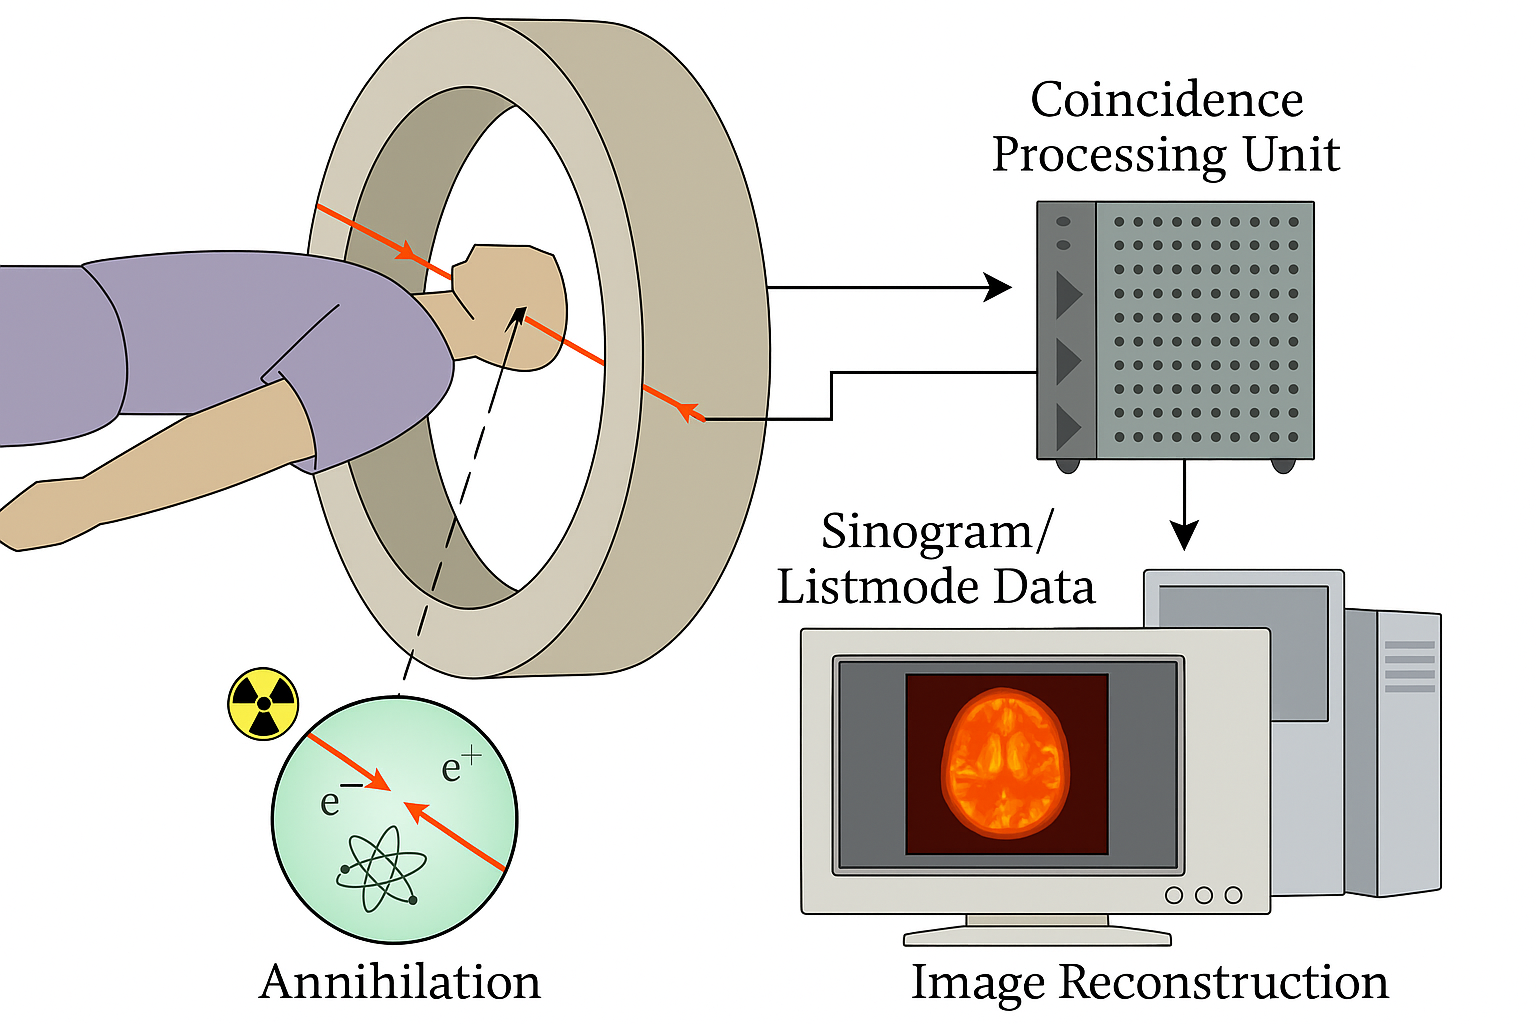
\includegraphics[width=0.85\textwidth]{bilder/petscan.png}
	\caption{Principle of positron emission tomography (PET): A radiopharmaceutical administered into the body emits a positron, which annihilates with an electron. Two gamma photons of \SI{511}{keV} each are emitted in opposite directions and registered by detectors in the PET ring. From the coincidence of signals, the point of origin is reconstructed.}
	\label{fig:pet_prinzip}
\end{figure}
\begin{tcolorbox}[didaktikbox, title=Concept: Annihilation]
	\label{box:annihilation}
	\small
	In \textbf{annihilation}, a particle and its antiparticle collide and annihilate each other. Their mass is fully converted into energy – usually in the form of photons. In PET, annihilation of an electron with a positron produces a photon pair of \SI{511}{keV} each.
\end{tcolorbox}
\vspace{1em}
\begin{tcolorbox}[didaktikbox, title=Concept: Radiopharmaceutical]
	\label{box:radiopharmakon}
	\small
	A \textbf{radiopharmaceutical} is a radioactively labeled compound administered specifically into the body. In PET, for example, [\textsuperscript{18}F]FDG is used – a sugar-like substance that accumulates in metabolically active tissues (such as tumors). The positrons produced there provide the image signal through annihilation.
\end{tcolorbox}

\subsubsection{Optical Tomography and Fluorescence Imaging}

In contrast to ionizing radiation, these techniques rely on visible or near-infrared light.

\textbf{Diffuse optical tomography (DOT)}\index{Diffuse optical tomography (DOT)} uses light sources and detectors on the skin surface. Photons penetrate the tissue, are scattered and absorbed. From the light distribution, the optical properties inside can be reconstructed.

\textbf{Fluorescence imaging}\index{Fluorescence imaging} employs substances (fluorophores\index{Fluorophore}) that are excited by light and re-emit at a different wavelength. This method allows, for example, the visualization of molecular processes or tumor markers.
\vspace{1em}
\begin{tcolorbox}[didaktikbox, title=Advantage of Optical Methods]
	\label{box:optisches Verfahren}
	\small
	Optical methods are non-invasive, free of ionizing radiation, and are particularly suitable for surface and functional imaging – e.g., in infants, neurodiagnostics, or molecular imaging.
\end{tcolorbox}

\subsubsection{Lasers in Surgery and Diagnostics}

Lasers\index{Laser} are used both for \textbf{imaging} and for \textbf{tissue interaction}:

\begin{itemize}
	\item \textbf{Diagnostic:} Confocal laser scanning microscopy\index{Confocal laser scanning microscopy}, optical coherence tomography (OCT)\index{Optical coherence tomography (OCT)}, spectroscopy\index{Spectroscopy}.
	\item \textbf{Surgical:} Tissue cutting, coagulation, ablation – depending on wavelength, pulse duration, and power.
\end{itemize}

Laser surgery\index{Laser surgery} exploits the precise focusing of photons for targeted tissue treatment without mechanical stress. Typical applications are:

\begin{itemize}
	\item Ophthalmology\index{Ophthalmology} (e.g., LASIK\index{LASIK}),
	\item Dermatology\index{Dermatology} (e.g., tattoo removal\index{Tattoo removal}),
	\item Tumor surgery\index{Tumor surgery} (precise cuts with minimal blood loss).
\end{itemize}

\begin{tcolorbox}[hinweisbox, title=Laser Parameters]
	\label{box:laserparameter}
	\small
	The effect of a laser strongly depends on its wavelength, pulse duration, energy, and focusing. Short pulses with high power allow precise cuts without damaging the surrounding tissue.
\end{tcolorbox}
\newpage
\noindent
\begin{figure}[H]
	\centering
	\includegraphics[width=0.85\textwidth]{bilder/oct.png}
	\caption{Schematic representation of optical coherence tomography (OCT): Light from a broadband source is split by a beam splitter. One part hits a movable reference mirror (reference arm), the other the tissue to be examined (sample). The reflected light portions interfere, and from the interference patterns the depth profile is reconstructed. The result is a high-resolution image, e.g., of the retina.}
	\label{fig:oct_prinzip}
\end{figure}

\begin{tcolorbox}[didaktikbox, title=Didactic Explanation: Interference in OCT]
	\label{box:interferenz_oct}
	\small
	\textbf{Interference} occurs when two light waves overlap – depending on the phase, they either reinforce or cancel each other. In OCT, this property is used to determine the position of reflecting structures in tissue with high precision.
	
	Only when the optical path lengths in the \emph{sample arm} and the \emph{reference arm} are nearly equal does an interference signal occur. From the measured intensity as a function of the reference arm position, an \textbf{A-scan} – a depth profile along a line in the tissue – is obtained.
	
	By laterally shifting the measurement beam, many A-scans next to each other are recorded, which together form a \textbf{B-scan} (2D cross-section). This produces a detailed image of the examined tissue – e.g., of the retina.
\end{tcolorbox}

\subsection{Photons in Communication}
\index{Photons in communication}
\index{Data transmission}
\index{Quantum communication}

Photons form the backbone of modern data transmission – both in classical fiber optic networks and in future quantum-based systems. The low-loss propagation of light in optical media, combined with high bandwidth and low latency, makes photonic communication technology a decisive factor in global information infrastructure.

\subsubsection{Optical Fiber and Optical Networks}
\index{Optical fiber}
\index{Optical networks}
\index{Total internal reflection}
\index{Wavelength division multiplexing}
\index{DWDM}
\index{EDFA}

\textbf{Optical fibers} guide light by total internal reflection in a thin quartz core. Photons can thus be transmitted over distances of several hundred kilometers with minimal attenuation.

Advantages:
\begin{itemize}
	\item extremely high data rates (terabits/s),
	\item immunity to electromagnetic interference,
	\item low attenuation (e.g., \SI{0.2}{dB/km} at \SI{1550}{nm}).
\end{itemize}

\textbf{Optical networks} use wavelength division multiplexing (DWDM), amplifiers (EDFAs), and modulated laser systems to transmit large amounts of data in parallel and efficiently – from backbone networks to fiber-to-the-home connections.
\vspace{1em}
\begin{tcolorbox}[physikbox, title=Total Internal Reflection in Optical Fibers]
	\label{box:glasfaser}
	\small
	Light guidance in an optical fiber is based on total internal reflection at the interface between the higher-refractive-index core and the cladding. The critical angle determines whether the light remains “trapped” inside the core.
\end{tcolorbox}
\newpage
\noindent
\begin{figure}[H]
	\centering
	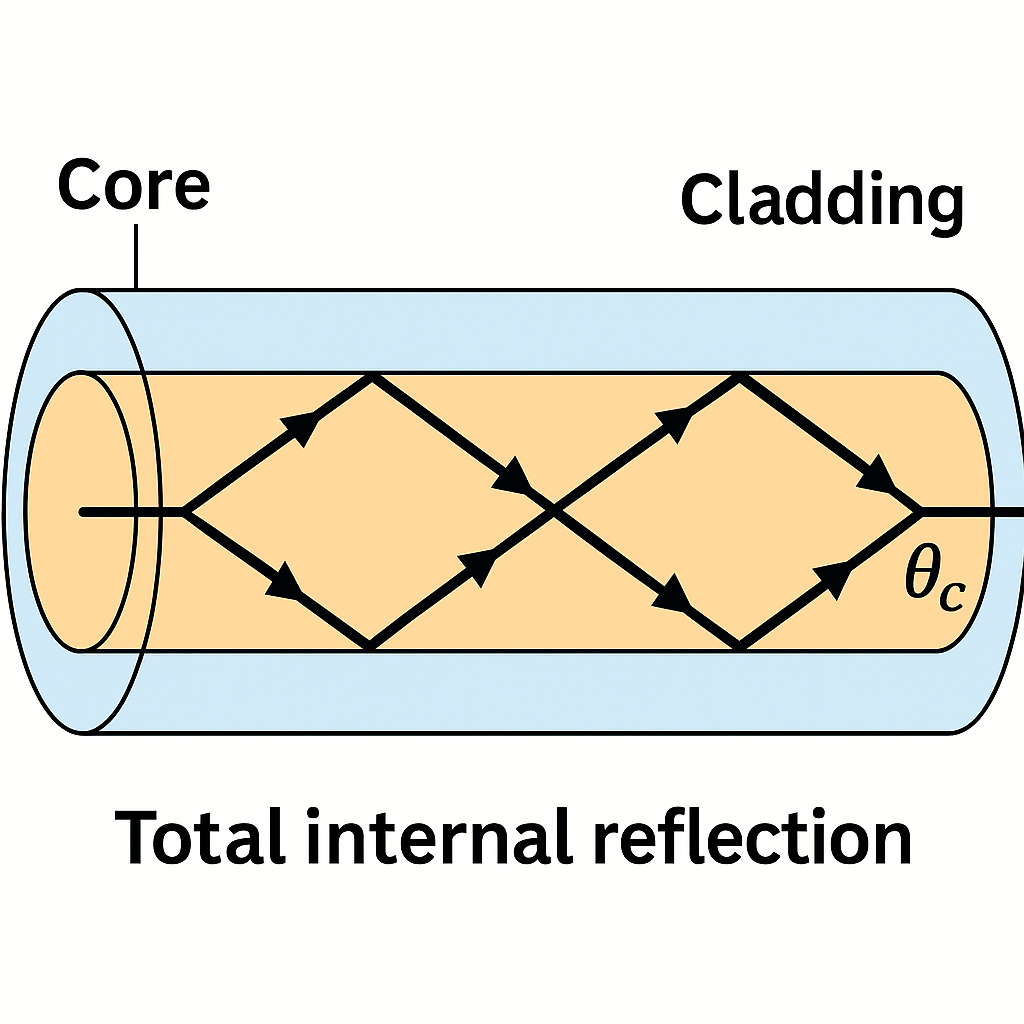
\includegraphics[width=0.8\textwidth]{bilder/glasfaser.png}
	\caption{Schematic illustration of total internal reflection in an optical fiber: Light (photons) is guided in the higher-index core and fully reflected at the interface with the cladding. This keeps the light “trapped” in the core even over long distances.}
	\label{fig:totalreflexion}
\end{figure}
\subsubsection{Quantum Communication and QKD}\index{Quantum communication}\index{QKD}\index{Photons!Quantum communication}\index{Polarization!Photons}\index{Entanglement!Photons}

\textbf{Quantum communication} exploits quantum states of photons – such as polarization or entanglement – to transmit information in a way that is absolutely secure against eavesdropping.

\textbf{QKD (Quantum Key Distribution)} is a practical application: Two parties (Alice and Bob) exchange a secret key. Any eavesdropping attempt (Eve) inevitably alters the quantum state of the photons and can thus be detected.
\newpage
\noindent
\begin{tcolorbox}[didaktikbox, title=What Makes QKD Secure?] \index{QKD!Security}
	\label{box:qkd}
	\small
	The security relies on two quantum-physical principles:
	\begin{itemize}
		\item \textbf{No-cloning theorem:} Unknown quantum states cannot be perfectly copied.
		\item \textbf{Measurement disturbance:} Any measurement affects the state – an eavesdropping attempt measurably disturbs the system.
	\end{itemize}
\end{tcolorbox}

\textbf{BB84} is the first and best-known QKD protocol. It uses random polarizations and basis changes to generate a key, which is then verified over a classical channel.

\vspace{1em}
\begin{tcolorbox}[didaktikbox, title={How Does QKD Work (e.g., BB84)?}] \index{QKD!BB84}\index{Quantum communication!BB84}
	\label{box:wie funktioniert QKD}
	\small
	In the BB84 protocol, Alice sends single photons whose polarization is randomly chosen – e.g., horizontal ($\rightarrow$), vertical ($\uparrow$), diagonal ($\searrow$), or anti-diagonal ($\nwarrow$). Bob also measures in random bases.
	
	Only when sender and receiver bases match does a valid bit result. After the exchange, Alice and Bob (publicly) compare the bases used and keep only the matching ones. From these bits, the key is generated.
	
	If a photon is intercepted, its polarization changes – allowing Alice and Bob to detect disturbances in the key and reveal eavesdropping attempts.
\end{tcolorbox}

\subsubsection{Photonic Chips and Future Systems}\index{Photonic chips}\index{Silicon photonics}\index{Photons!Photonic chips}\index{Data processing!Photonic}\index{Logic systems!Photonic}

With the advent of \textbf{photonic chips}, light signals are no longer guided solely through optical fibers but directly through integrated optical circuits. These enable:

\begin{itemize}
	\item compact, energy-efficient data processing,
	\item light-based logic and modulation systems,
	\item new concepts for neural networks and AI accelerators.
\end{itemize}

Photonic chips combine lasers, modulators, waveguides, and detectors on a single substrate – often silicon photonics.
\newpage
\noindent
\begin{tcolorbox}[hinweisbox, title=Future of Photonic Communication] \index{Photon-based communication}
	\label{box:Zukunft Kommunikation}
	\small
	Photon-based communication is not only faster than classical electronics – it will become a prerequisite for secure quantum networks, light-based processors, and global, tap-proof communication.
\end{tcolorbox}

\subsection{Photons in Astronomical Observation}\index{Astronomy!Photons}\index{Photons!Astronomy}\index{Photons!Astronomical observation}

The observation of photons from space is the foundation of modern astronomy. Since photons – unlike, for example, gravitational waves or neutrinos – are comparatively easy to detect, they provide most of our information about the universe. Whether visible light, radio waves, or high-energy gamma rays – every photon reaching Earth carries a message from space and time.

\subsubsection{Detection of Photons from Space}\index{Detection!Photons}\index{Photons!Detection!Astronomical}

Telescopes and detectors on Earth and in space measure photons across various wavelength ranges:

\begin{itemize}
	\item \textbf{Optical range:} CCDs (charge-coupled devices), CMOS sensors
	\item \textbf{Infrared and radio:} Bolometers, radio telescopes
	\item \textbf{X-rays and gamma rays:} Space telescopes with scintillators and semiconductor detectors
\end{itemize}

The analysis of these photons provides information about temperature, motion (Doppler shift), composition, and distance of cosmic objects.

\vspace{1em}
\begin{tcolorbox}[physikbox, title=Why Don’t All Photons Reach Earth?] \index{Earth’s atmosphere!Photon absorption}\index{Photons!Earth’s atmosphere}
	\label{box:photonen auf erde}
	\small
	The Earth’s atmosphere is opaque to many wavelength ranges – especially UV, X-rays, and gamma rays. Therefore, corresponding telescopes must be positioned outside the atmosphere – e.g., in Earth orbit.
\end{tcolorbox}
\newpage
\noindent
\subsubsection{Adaptive Optics, Spectroscopy, and Telescopes}
\index{Adaptive optics}
\index{Spectroscopy}
\index{Telescopes}
\index{Interferometry}

\textbf{Telescopes} collect photons\index{Photon} and focus them onto detectors. Modern large telescopes (e.g., the VLT\index{Very Large Telescope (VLT)} or ELT\index{Extremely Large Telescope (ELT)}) use adaptive optics to improve image quality:

- \textbf{Adaptive optics} compensates for atmospheric distortions in real time using deformable mirrors.
- \textbf{Spectroscopy} disperses light into its wavelengths and allows the analysis of chemical composition, temperature, and motion of celestial bodies.
- \textbf{Interferometry} combines several telescopes into a virtual giant telescope with extremely high angular resolution.
\begin{figure}[H]
	\centering
	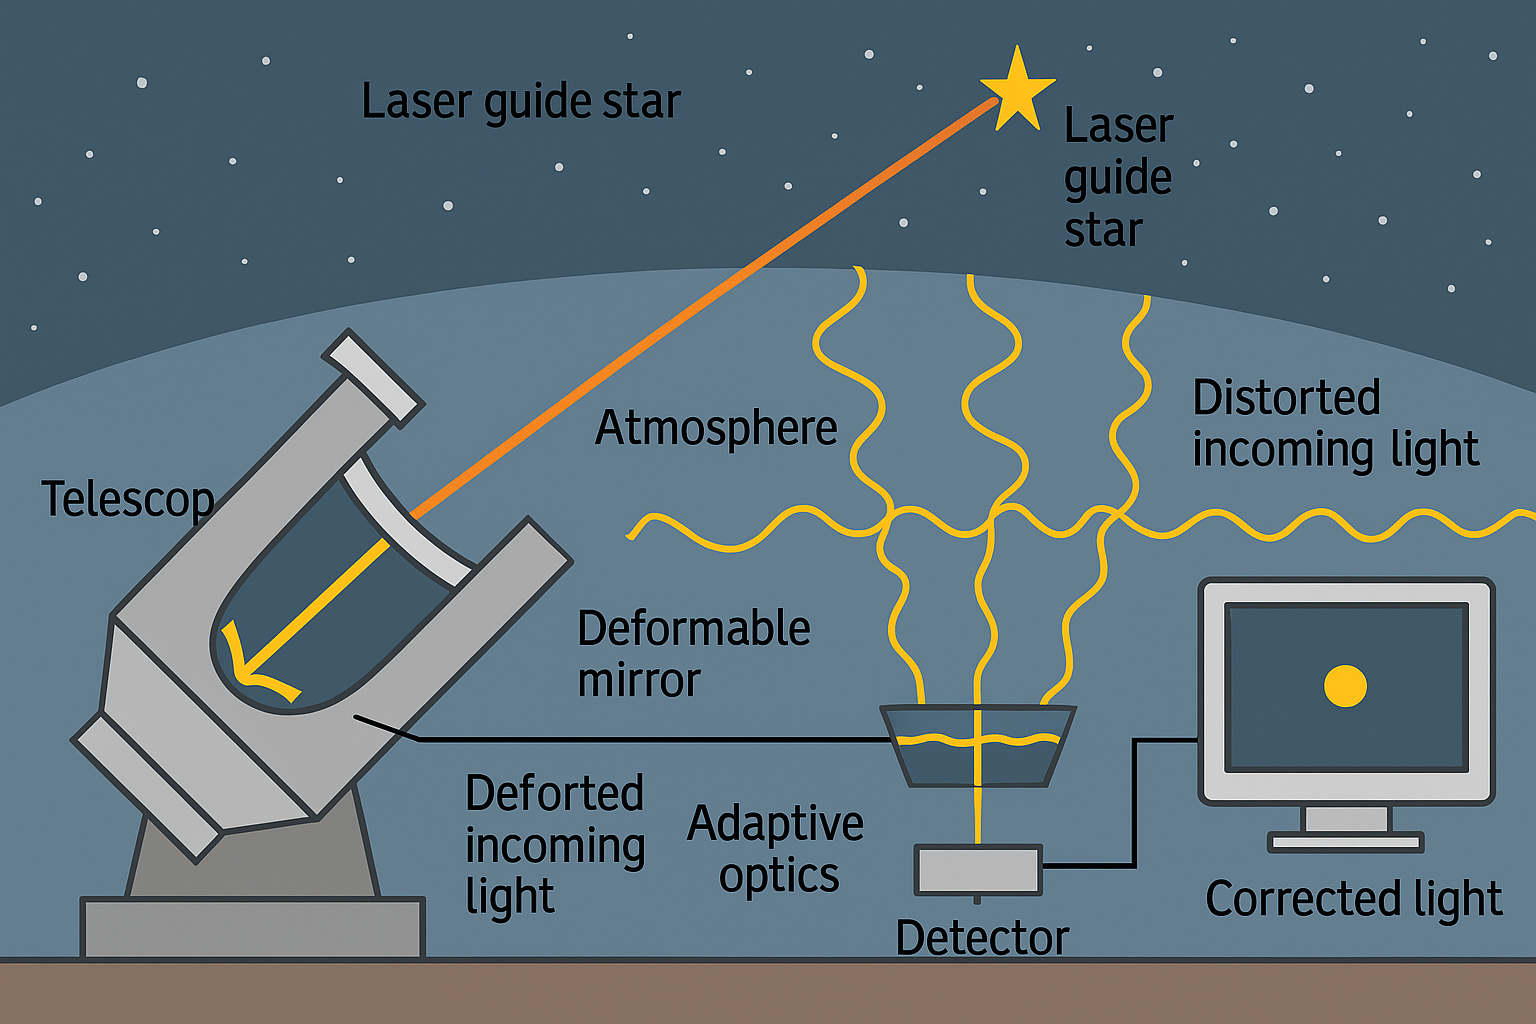
\includegraphics[width=0.9\textwidth]{bilder/Teleskop.png}
	\caption{Schematic illustration of a telescope with adaptive optics. A wavefront sensor analyzes distortions caused by the atmosphere. A deformable mirror surface corrects these in real time, producing a sharp image.}
	\label{fig:adaptive_optik}
\end{figure}

\begin{tcolorbox}[didaktikbox, title=What Does a Spectrum Show?]
	\label{box:was zeigt spektrum}
	\small
	A \textbf{spectrum}\index{Spectrum} is the distribution of photon intensity as a function of wavelength. Typical features include:
	\begin{itemize}
		\item \textbf{Emission lines}\index{Emission lines} $\rightarrow$ hot, radiating gases,
		\item \textbf{Absorption lines}\index{Absorption lines} $\rightarrow$ cold gases in front of hot sources,
		\item \textbf{Redshift}\index{Redshift} $\rightarrow$ motion of the object away from the observer.
	\end{itemize}
\end{tcolorbox}
\begin{figure}[H]
	\centering
	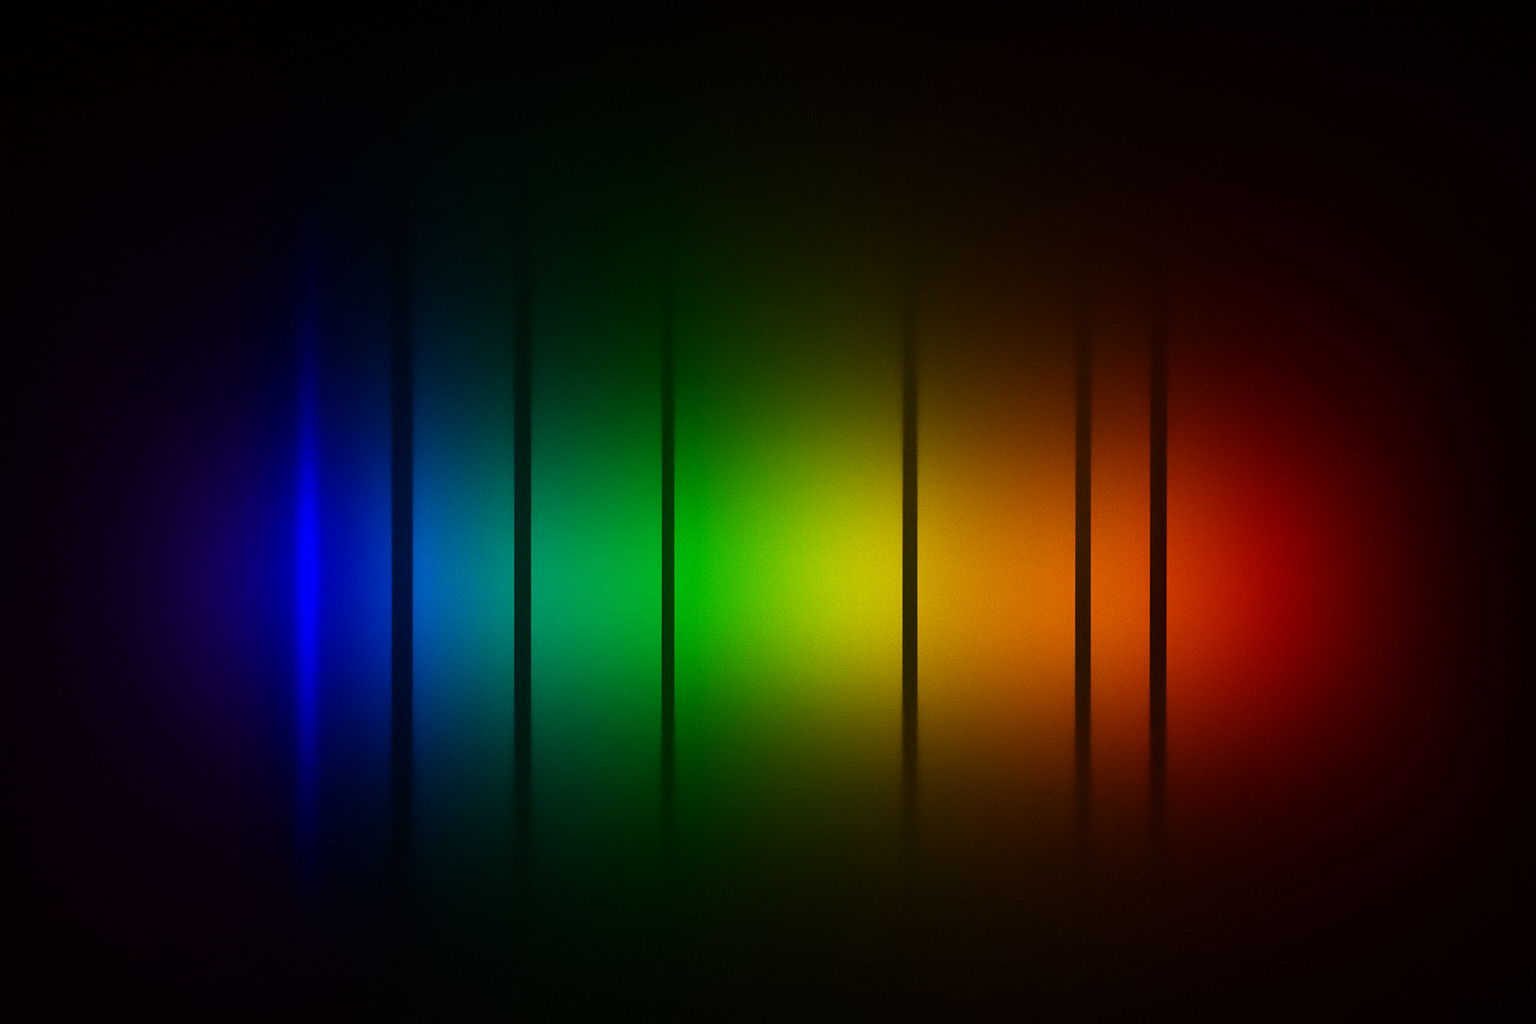
\includegraphics[width=0.9\textwidth]{bilder/emissionslinien.png}
	\caption{Emission spectrum of glowing hydrogen gas.}
	\label{fig:emission_hydrogen}
\end{figure}

\begin{tcolorbox}[physikbox, title=Spectral Lines and Redshift]
	\label{box:spektrallinien}
	\small
	\begin{itemize}
		\item \textbf{Emission lines} arise when atoms emit specific photons. These lines are bright and characteristic of the respective element\index{Element spectrum}.
		\item \textbf{Absorption lines} occur when photons of certain frequencies are absorbed by a gas through which the light passes – they then appear missing in the spectrum.
		\item \textbf{Redshift:} When a light source moves away, all lines shift to longer wavelengths – toward red. This is used to measure cosmic motion\index{Cosmic expansion}.
	\end{itemize}
\end{tcolorbox}

\subsubsection{Photons in Gravitational Wave Astronomy}
\index{Gravitational wave astronomy}
\index{Gravitational waves}
\index{Photon}
\index{Interferometer}
\index{LIGO}
\index{Virgo}

Gravitational waves are fundamental distortions of spacetime\index{Spacetime} – triggered by accelerated masses, such as the merger of black holes\index{Black hole}. They are not electromagnetic waves and are not made of photons. Nevertheless, it is precisely photons that enable their detection: as precise probes in highly sensitive interferometers.

\vspace{0.5em}
\textbf{LIGO, Virgo, and other gravitational wave detectors} use kilometer-scale laser interferometers to measure minute changes in spacetime. Laser beams (consisting of coherent photons) are sent into two perpendicular arms, reflected by mirrors, and recombined at the output. A passing gravitational wave slightly changes the arm lengths – and thus the interference pattern.

\vspace{1em}
\begin{tcolorbox}[physikbox, title=Photons as a Tool for Measuring Spacetime Curvature]
	\label{box:messwerkzeug}
	\small
	Laser interferometers such as LIGO use photons to detect differences in arm length as small as \SI{1e-19}{m} – about a thousand times smaller than a proton\index{Proton}. The time difference a photon needs to traverse the two arms changes measurably due to a passing gravitational wave.
\end{tcolorbox}

This technique relies on the interference\index{Interference} of coherent light waves. When the two beams are recombined after traveling through the arms, constructive or destructive interference occurs depending on the phase shift. Even the smallest changes in optical path length affect this pattern. In this way, even minute curvatures of spacetime can be detected.

\vspace{0.5em}
Thanks to this photon-based precision measurement, events such as black hole mergers, neutron star collisions\index{Neutron star}, or traces of the cosmic gravitational background\index{Cosmic gravitational background} have been experimentally confirmed. Photons thus make visible what would otherwise lie beyond direct observation – further evidence of their central role in modern physics.
\newpage
\noindent
\vspace{1em}
\begin{tcolorbox}[didaktikbox, title=How Does an Interferometer Work? \label{box:interferometer}]
	\small
	An interferometer uses the principle of superposition (interference) of light waves to make the smallest length differences visible. 
	
	\begin{itemize}
		\item A laser beam\index{Laser} is split into two partial beams using a beam splitter.
		\item These travel along two perpendicular arms to mirrors, are reflected, and recombined.
		\item If the optical path lengths of the two arms are exactly equal, the waves cancel each other partly or completely – the interference pattern is constant.
		\item If one arm length changes slightly (e.g., due to a gravitational wave), the phase of one wave shifts, and the interference pattern measurably changes.
	\end{itemize}
	
	Thus, even length changes smaller than an atom’s diameter can be detected by analyzing the light intensity at the detector. Light serves as a precise “measuring stick” in space.
\end{tcolorbox}

\vspace{1em}
\begin{tcolorbox}[didaktikbox, title=Why Are Photons So Precisely Measurable? \label{box:photonen_genau}]
	\small
	Photons are ideal measurement tools – for several reasons:
	
	\begin{itemize}
		\item \textbf{High coherence:} Laser light consists of coherent photons – i.e., waves with exactly the same frequency and stable phase. This enables extremely sensitive interference effects.
		\item \textbf{Low interaction:} Photons hardly interact with matter. This allows long propagation paths without disturbance or deflection.
		\item \textbf{Quantum nature:} Single photons are discrete quantum objects\index{Quantum nature}. Their detection produces clear, countable signals – ideal for precise time or position measurements.
		\item \textbf{Speed of light as a constant:} The velocity of photons in a vacuum is constant\index{Speed of light}. This makes them natural “standards” for time and length.
	\end{itemize}
	
	These properties make photons indispensable in modern metrology – from interferometers to quantum sensors\index{Quantum sensor} to optical atomic clocks\index{Optical atomic clock}.
\end{tcolorbox}

\subsubsection{Conclusion}

Photons are not only central objects of modern physics but also indispensable tools in science, engineering, medicine, and communication. This chapter has shown how diverse and precise photons can be controlled, generated, and detected:

\begin{itemize}
	\item In \textbf{laser technology}\index{Laser technology}, stimulated emission and coherent light amplification enable applications ranging from materials processing to quantum optics\index{Quantum optics}.
	\item \textbf{Photon detectors}\index{Photon detector} such as SPADs\index{SPAD} or PMTs\index{Photomultiplier (PMT)} allow single-photon counting with high quantum efficiency\index{Quantum efficiency} – a foundation for quantum technologies\index{Quantum technology} and precise imaging.
	\item In \textbf{medical diagnostics}\index{Medical diagnostics}, photons are used for imaging with high spatial resolution and minimal exposure – from X-rays\index{X-rays} to fluorescence microscopy\index{Fluorescence microscopy}.
	\item \textbf{Optical communication}\index{Optical communication} uses photons for fast, low-loss, and secure data transmission – in fibers\index{Optical fiber} as well as in quantum communication systems\index{Quantum communication}.
	\item In \textbf{astronomical observation}\index{Astronomy}, photons provide crucial information about the structure, motion, and composition of the universe – up to the detection of gravitational waves through interferometric measurement.
\end{itemize}

The ability to deliberately generate, guide, and measure single photons marks a technological turning point: From classical applications to quantum information technology\index{Quantum information technology}, the photon opens new horizons – in research, industry, and society.
